\setAuthor{Tundmatu autor}
\setRound{lõppvoor}
\setYear{2004}
\setNumber{G 9}
\setDifficulty{1}
\setTopic{Teema}

\prob{Peeglid}
Ekraan, kaks peeglit ning koherentse monokromaatilise kiirguse allikas (kiiratav lainepikkus $\lambda$) on paigutatud nii, nagu näidatud joonisel. Valgusallikast jõuab ekraanile vaid peegeldunud valgus. Peeglite normaalide vaheline nurk on $2 \alpha$. Peeglite puutepunkti ning valgusallika vaheline kaugus on $a$ ning valgusallika kaugus ekraanist on samuti $a$. On teada, et punkti $O$ lähedusse tekib interferentsimuster, kus järjestikuste tumedate triipude vaheline kaugus on $d$. Leida lainepikkus $\lambda .$ Eeldada, et $a \gg d$.
\begin{center}
	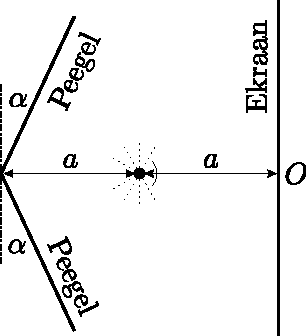
\includegraphics[width=0.6\linewidth]{2004-v3g-09-yl.pdf}
\end{center}

\hint

\solu
Leiame valgusallika kujutised peeglites. Punkti $O$ ümbrusse langevat valgust võime siis vaadelda kujutistest kiiratud valguse superpositsioonina. Leiame järgnevalt $\sin \phi .$ Antud geomeetrilisest konstruktsioonist saame:
$$
x=2 a \cos \alpha \sin \alpha, \quad y=2 a \cos \alpha \cos \alpha+a
$$
$\tan \phi=\frac{x}{y}=\frac{2 a \cos \alpha \sin \alpha}{2 a \cos \alpha \cos \alpha+a}, \quad \sin \phi=\frac{1}{\sqrt{1+(\cot \phi)^{2}}}$,
$\sin \phi=\left[1+\left(\frac{2 a \cos \alpha \cos \alpha+a}{2 a \cos \alpha \sin \alpha}\right)^{2}\right]^{-\frac{1}{2}}=\left[1+\left(\frac{\cos \alpha+1 /(2 \cos \alpha)}{\sin \alpha}\right)^{2}\right]^{-\frac{1}{2}}$
$=\frac{\sin \alpha}{\sqrt{\sin ^{2} \alpha+\left(\cos \alpha+1 /(2 \cos \alpha)^{2}\right)}}=\frac{\sin \alpha}{\sqrt{2+1 /\left(4 \cos ^{2} \alpha\right)}}=\frac{\sin 2 \alpha}{\sqrt{8 \cos ^{2} \alpha+1}}$

\begin{center}
	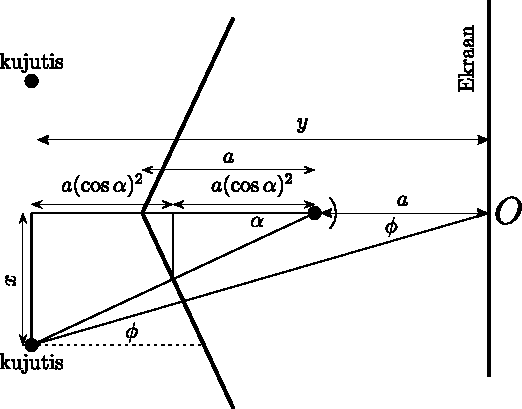
\includegraphics[width=0.8\linewidth]{2004-v3g-09-lah.pdf}
\end{center}

Olgu punkti $O$ läheduses mingis punktis $M$ interferentsi miinimum. Kui liiguksime sellest punktist $d$ võrra ülespoole, siis alumisest kujutisest tuleva valguse teekond pikeneb $d \sin \phi$ vōrra ning ülemisest kujutisest tuleva valguse teekond lüheneb $d \sin \phi$ võrra. Seega saame punktiga $M$ võrreldes käiguvahe $2 d \sin \phi$. Sellele vastab miinimum juhul kui $\lambda=2 d \sin \phi$. Seega saamegi vastuseks
\[
\lambda=\frac{2 d \sin 2 \alpha}{\sqrt{8 \cos ^{2} \alpha+1}}
\]

\probend